
\documentclass[convert={outext=.jpg}]{standalone}
\usepackage{ulem,tikz}
\usetikzlibrary{positioning}

\begin{document}
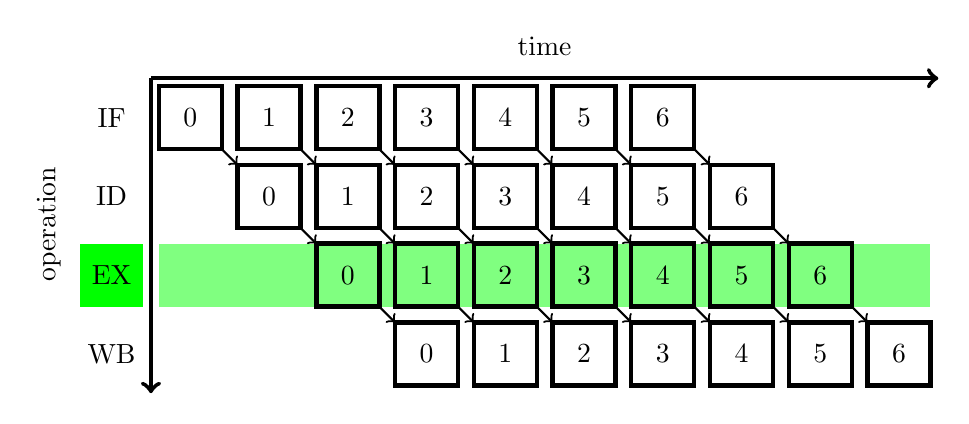
\begin{tikzpicture}[ultra thick]
  \draw [->] (0, 0) -- (10,0) node[midway, label={time}] {};
  \path (-1, 0) -- (-1,-4) node[midway,
  label={[rotate=90]operation}] {};
  \draw [->] (0, 0) -- (0,-4);
  \fill[green] (-0.9,-2.1) rectangle ++(0.8,-0.8);
  \fill[green!50!white] (0.1,-2.1) rectangle ++(9.8,-0.8);
  \path (-0.5,-0.5) node {IF}
      ++(0,-1) node {ID}
      ++(0,-1) node {EX}
      ++(0,-1) node {WB};

  \foreach \x in {0,...,6}
    {%
      \draw (\x, 0)
       +(0.1,-0.1) rectangle +(0.9,-0.9) node[midway]{\x}
       ++(1,-1)
       +(0.1,-0.1) rectangle +(0.9,-0.9) node[midway]{\x}
       ++(1,-1)
       +(0.1,-0.1) rectangle +(0.9,-0.9) node[midway]{\x}
       ++(1,-1)
       +(0.1,-0.1) rectangle +(0.9,-0.9) node[midway]{\x};
      \draw [thick,->] (\x, 0)    +(0.9,-0.9) -- +(1.1,-1.1);
      \draw [thick,->] (\x+1, -1) +(0.9,-0.9) -- +(1.1,-1.1);
      \draw [thick,->] (\x+2, -2) +(0.9,-0.9) -- +(1.1,-1.1);
    }%
\end{tikzpicture}
\end{document}
